\documentclass{standalone}
\usepackage{tikz}
\usetikzlibrary{patterns, positioning}

\begin{document}
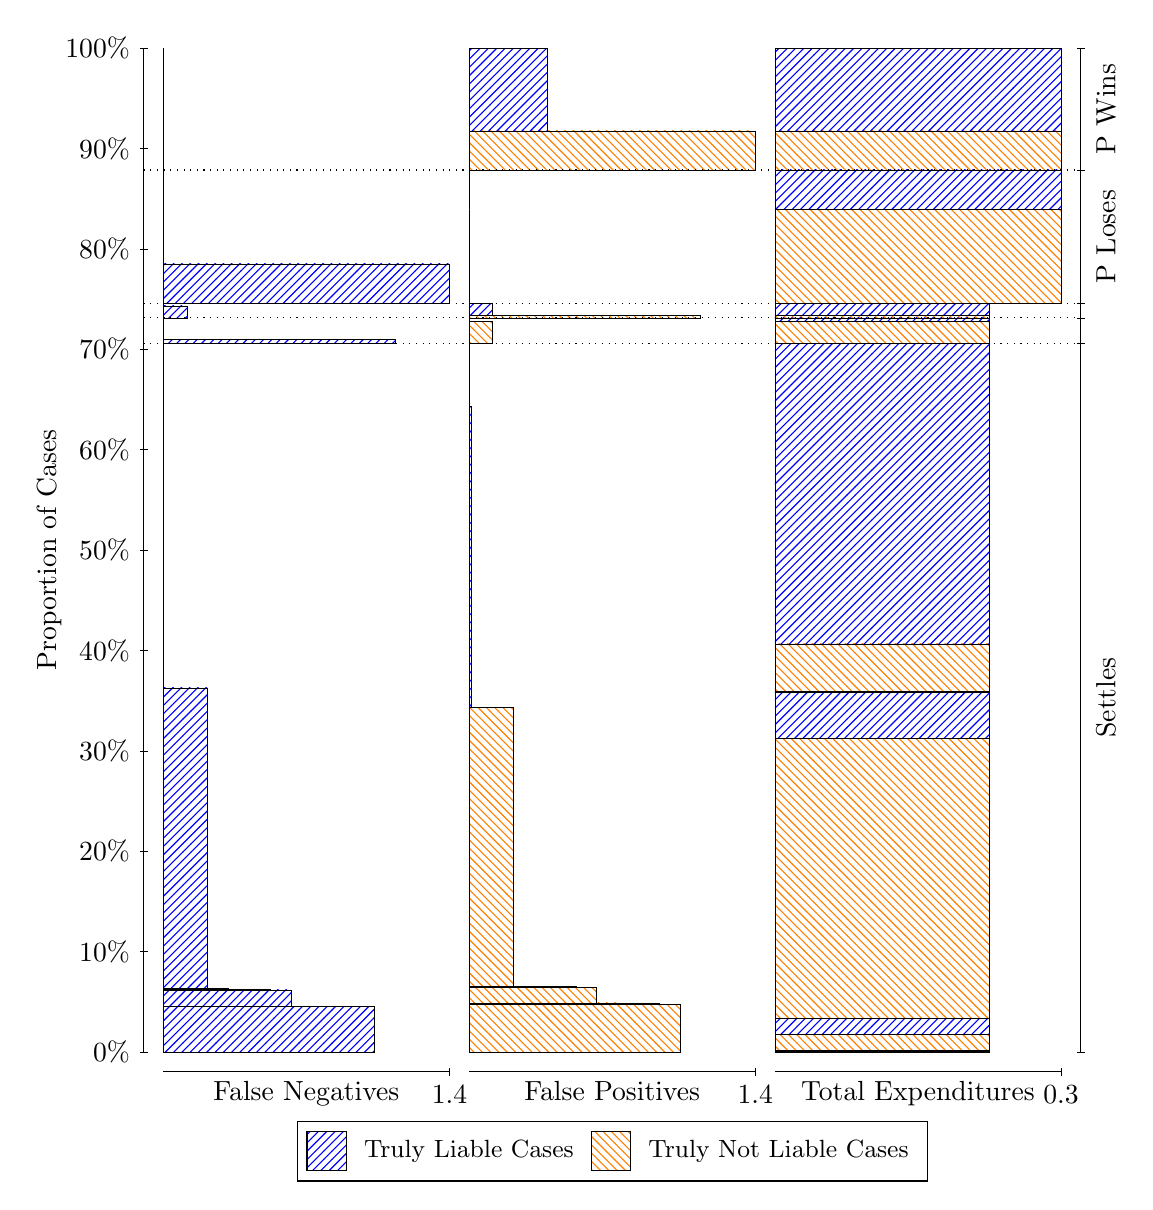
\begin{tikzpicture}
\draw[black, very thin] (1.5,1.75) -- (1.5,14.5);
\node[rotate=90, anchor=center] at (0.3, 8.125) {Proportion of Cases};
\draw[black, very thin] (1.45,1.75) -- (1.55,1.75);
\node[anchor=east] at (1.45, 1.75) {0\%};
\draw[black, very thin] (1.45,3.025) -- (1.55,3.025);
\node[anchor=east] at (1.45, 3.025) {10\%};
\draw[black, very thin] (1.45,4.3) -- (1.55,4.3);
\node[anchor=east] at (1.45, 4.3) {20\%};
\draw[black, very thin] (1.45,5.575) -- (1.55,5.575);
\node[anchor=east] at (1.45, 5.575) {30\%};
\draw[black, very thin] (1.45,6.85) -- (1.55,6.85);
\node[anchor=east] at (1.45, 6.85) {40\%};
\draw[black, very thin] (1.45,8.125) -- (1.55,8.125);
\node[anchor=east] at (1.45, 8.125) {50\%};
\draw[black, very thin] (1.45,9.4) -- (1.55,9.4);
\node[anchor=east] at (1.45, 9.4) {60\%};
\draw[black, very thin] (1.45,10.675) -- (1.55,10.675);
\node[anchor=east] at (1.45, 10.675) {70\%};
\draw[black, very thin] (1.45,11.95) -- (1.55,11.95);
\node[anchor=east] at (1.45, 11.95) {80\%};
\draw[black, very thin] (1.45,13.225) -- (1.55,13.225);
\node[anchor=east] at (1.45, 13.225) {90\%};
\draw[black, very thin] (1.45,14.5) -- (1.55,14.5);
\node[anchor=east] at (1.45, 14.5) {100\%};

\draw[black, very thin] (13.4,1.75) -- (13.4,14.5);
\draw[black, very thin] (13.35,1.75) -- (13.45,1.75);
\node[anchor=west] at (13.35, 1.75) {};
\draw[black, very thin] (13.35,10.753) -- (13.45,10.753);
\node[anchor=west] at (13.35, 10.753) {};
\draw[black, very thin] (13.35,11.073) -- (13.45,11.073);
\node[anchor=west] at (13.35, 11.073) {};
\draw[black, very thin] (13.35,11.26) -- (13.45,11.26);
\node[anchor=west] at (13.35, 11.26) {};
\draw[black, very thin] (13.35,12.951) -- (13.45,12.951);
\node[anchor=west] at (13.35, 12.951) {};
\draw[black, very thin] (13.35,14.5) -- (13.45,14.5);
\node[anchor=west] at (13.35, 14.5) {};

\draw[black, very thin, pattern color=blue, pattern=north east lines] (1.75,1.75) rectangle (4.4255,2.3246);
\draw[black, very thin, pattern color=blue, pattern=north east lines] (1.75,2.3246) rectangle (4.1612,2.3277);
\draw[black, very thin, pattern color=blue, pattern=north east lines] (1.75,2.3277) rectangle (3.897,2.3307);
\draw[black, very thin, pattern color=blue, pattern=north east lines] (1.75,2.3307) rectangle (3.6327,2.3337);
\draw[black, very thin, pattern color=blue, pattern=north east lines] (1.75,2.3337) rectangle (3.6327,2.3337);
\draw[black, very thin, pattern color=blue, pattern=north east lines] (1.75,2.3337) rectangle (3.3685,2.5389);
\draw[black, very thin, pattern color=blue, pattern=north east lines] (1.75,2.5389) rectangle (3.1042,2.5441);
\draw[black, very thin, pattern color=blue, pattern=north east lines] (1.75,2.5441) rectangle (2.84,2.5493);
\draw[black, very thin, pattern color=blue, pattern=north east lines] (1.75,2.5493) rectangle (2.5758,2.5546);
\draw[black, very thin, pattern color=blue, pattern=north east lines] (1.75,2.5546) rectangle (2.3115,6.3743);
\draw[black, very thin, pattern color=orange, pattern=north west lines] (1.75,6.3743) rectangle (1.75,10.753);
\draw[black, very thin, pattern color=blue, pattern=north east lines] (1.75,10.753) rectangle (4.6897,10.801);
\draw[black, very thin, pattern color=orange, pattern=north west lines] (1.75,10.801) rectangle (1.75,11.073);
\draw[black, very thin, pattern color=blue, pattern=north east lines] (1.75,11.073) rectangle (2.0473,11.226);
\draw[black, very thin, pattern color=orange, pattern=north west lines] (1.75,11.226) rectangle (1.75,11.26);
\draw[black, very thin, pattern color=blue, pattern=north east lines] (1.75,11.26) rectangle (5.3833,11.759);
\draw[black, very thin, pattern color=orange, pattern=north west lines] (1.75,11.759) rectangle (1.75,12.951);
\draw[black, very thin, pattern color=orange, pattern=north west lines] (1.75,12.951) rectangle (1.75,13.449);
\draw[black, very thin, pattern color=blue, pattern=north east lines] (1.75,13.449) rectangle (1.75,14.5);
\draw[black, very thin, pattern color=orange, pattern=north west lines] (5.6333,1.75) rectangle (8.3088,2.3573);
\draw[black, very thin, pattern color=orange, pattern=north west lines] (5.6333,2.3573) rectangle (8.0445,2.3628);
\draw[black, very thin, pattern color=orange, pattern=north west lines] (5.6333,2.3628) rectangle (7.7803,2.3684);
\draw[black, very thin, pattern color=orange, pattern=north west lines] (5.6333,2.3684) rectangle (7.5161,2.3739);
\draw[black, very thin, pattern color=orange, pattern=north west lines] (5.6333,2.3739) rectangle (7.2518,2.5752);
\draw[black, very thin, pattern color=orange, pattern=north west lines] (5.6333,2.5752) rectangle (6.9876,2.5788);
\draw[black, very thin, pattern color=orange, pattern=north west lines] (5.6333,2.5788) rectangle (6.7233,2.5825);
\draw[black, very thin, pattern color=orange, pattern=north west lines] (5.6333,2.5825) rectangle (6.4591,2.5861);
\draw[black, very thin, pattern color=orange, pattern=north west lines] (5.6333,2.5861) rectangle (6.1948,6.1285);
\draw[black, very thin, pattern color=blue, pattern=north east lines] (5.6333,6.1285) rectangle (5.6664,9.9482);
\draw[black, very thin, pattern color=blue, pattern=north east lines] (5.6333,9.9482) rectangle (5.6333,10.753);
\draw[black, very thin, pattern color=orange, pattern=north west lines] (5.6333,10.753) rectangle (5.9306,11.025);
\draw[black, very thin, pattern color=blue, pattern=north east lines] (5.6333,11.025) rectangle (5.6333,11.073);
\draw[black, very thin, pattern color=orange, pattern=north west lines] (5.6333,11.073) rectangle (8.573,11.107);
\draw[black, very thin, pattern color=blue, pattern=north east lines] (5.6333,11.107) rectangle (5.9306,11.26);
\draw[black, very thin, pattern color=orange, pattern=north west lines] (5.6333,11.26) rectangle (5.6333,12.452);
\draw[black, very thin, pattern color=blue, pattern=north east lines] (5.6333,12.452) rectangle (5.6333,12.951);
\draw[black, very thin, pattern color=orange, pattern=north west lines] (5.6333,12.951) rectangle (9.2667,13.449);
\draw[black, very thin, pattern color=blue, pattern=north east lines] (5.6333,13.449) rectangle (6.6242,14.5);
\draw[black, very thin, pattern color=orange, pattern=north west lines] (9.5167,1.75) rectangle (12.242,1.7611);
\draw[black, very thin, pattern color=blue, pattern=north east lines] (9.5167,1.7611) rectangle (12.242,1.7717);
\draw[black, very thin, pattern color=orange, pattern=north west lines] (9.5167,1.7717) rectangle (12.242,1.973);
\draw[black, very thin, pattern color=blue, pattern=north east lines] (9.5167,1.973) rectangle (12.242,2.1782);
\draw[black, very thin, pattern color=orange, pattern=north west lines] (9.5167,2.1782) rectangle (12.242,5.7314);
\draw[black, very thin, pattern color=blue, pattern=north east lines] (9.5167,5.7314) rectangle (12.242,6.3151);
\draw[black, very thin, pattern color=orange, pattern=north west lines] (9.5167,6.3151) rectangle (12.242,6.3206);
\draw[black, very thin, pattern color=blue, pattern=north east lines] (9.5167,6.3206) rectangle (12.242,6.3259);
\draw[black, very thin, pattern color=orange, pattern=north west lines] (9.5167,6.3259) rectangle (12.242,6.9331);
\draw[black, very thin, pattern color=blue, pattern=north east lines] (9.5167,6.9331) rectangle (12.242,10.753);
\draw[black, very thin, pattern color=orange, pattern=north west lines] (9.5167,10.753) rectangle (12.242,11.025);
\draw[black, very thin, pattern color=blue, pattern=north east lines] (9.5167,11.025) rectangle (12.242,11.073);
\draw[black, very thin, pattern color=orange, pattern=north west lines] (9.5167,11.073) rectangle (12.242,11.107);
\draw[black, very thin, pattern color=blue, pattern=north east lines] (9.5167,11.107) rectangle (12.242,11.26);
\draw[black, very thin, pattern color=orange, pattern=north west lines] (9.5167,11.26) rectangle (13.15,12.452);
\draw[black, very thin, pattern color=blue, pattern=north east lines] (9.5167,12.452) rectangle (13.15,12.951);
\draw[black, very thin, pattern color=orange, pattern=north west lines] (9.5167,12.951) rectangle (13.15,13.449);
\draw[black, very thin, pattern color=blue, pattern=north east lines] (9.5167,13.449) rectangle (13.15,14.5);
\draw[black, dotted] (1.5,10.753) -- (13.4,10.753);
\draw[black, dotted] (1.5,11.073) -- (13.4,11.073);
\draw[black, dotted] (1.5,11.26) -- (13.4,11.26);
\draw[black, dotted] (1.5,12.951) -- (13.4,12.951);
\draw[black, very thin] (1.75,1.5) -- (5.3833,1.5);
\node[anchor=north] at (3.5667, 1.5) {False Negatives};
\draw[black, very thin] (5.3833,1.45) -- (5.3833,1.55);
\node[anchor=north] at (5.3833, 1.45) {1.4};

\draw[black, very thin] (5.6333,1.5) -- (9.2667,1.5);
\node[anchor=north] at (7.45, 1.5) {False Positives};
\draw[black, very thin] (9.2667,1.45) -- (9.2667,1.55);
\node[anchor=north] at (9.2667, 1.45) {1.4};

\draw[black, very thin] (9.5167,1.5) -- (13.15,1.5);
\node[anchor=north] at (11.333, 1.5) {Total Expenditures};
\draw[black, very thin] (13.15,1.45) -- (13.15,1.55);
\node[anchor=north] at (13.15, 1.45) {0.3};

\node[black, centered, rotate=90] at (13.72, 6.2514) {Settles};


\node[black, centered, rotate=90] at (13.72, 12.105) {P Loses};
\node[black, centered, rotate=90] at (13.72, 13.725) {P Wins};

\draw (7.449999999999999,1.5) node[draw=none] (baseCoordinate) {};
\begin{scope}[align=center]
        \matrix[scale=0.5, draw=black, below=0.5cm of baseCoordinate, nodes={draw}, column sep=0.1cm]{
            \node[rectangle, draw, minimum width=0.5cm, minimum height=0.5cm, pattern=north east lines, pattern color=blue] {}; &
            \node[draw=none, font=\small] (B) {Truly Liable Cases}; &
            \node[rectangle, draw, minimum width=0.5cm, minimum height=0.5cm, pattern=north west lines, pattern color=orange] {}; &
            \node[draw=none, font=\small] (B) {Truly Not Liable Cases}; \\
            };
\end{scope}

\end{tikzpicture}
\end{document}